\subsubsection{UC6.2 - Personalizzazione Heat Map}
\begin{figure}[h]
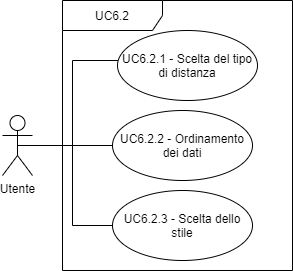
\includegraphics[width=9cm]{Section/Images/UC6.2.png}
\centering
\caption{UC6.2 - Personalizzazione Heat Map}
\end{figure}
\begin{itemize}
	\item \textbf{Attore primario}: Utente;
	
	\item \textbf{Precondizioni}: L'utente ha scelto il grafico \textit{Heat Map} [UC5.2];
	
	\item \textbf{Postcondizioni}: Il grafico viene aggiornato con le personalizzazioni impostate dall'utente.
	
	\item \textbf{Scenario principale}: L'utente decide:
	
\begin{enumerate}
\item Il tipo di distanza per il calcolo [UC6.2.1];
\item Se ordinare i dati e opzionalmente inserire il \glo{dendrogramma} [UC6.2.2];
\item Alcuni stili del grafico [UC6.2.3].
\end{enumerate}	
		
\end{itemize}
